\documentclass[a4paper,12pt]{article}
\renewcommand{\familydefault}{\sfdefault}


%                   %
% Package importing %
%                   %

% Images, wraping
\usepackage{graphicx}
\usepackage{wrapfig}
\usepackage{float}

% Allow more floats per page
\setcounter{topnumber}{8}
\setcounter{bottomnumber}{8}
\setcounter{totalnumber}{8}

% Doc margins
\usepackage[left = 50pt, right = 50pt, top = 60pt, bottom = 60pt]{geometry}

% Line spacing
\usepackage[utf8]{inputenc}
\usepackage[english]{babel}

\setlength{\parindent}{0pt}

% Hyperlinks
\usepackage{hyperref}
\hypersetup {
	colorlinks = true,
	linkcolor = cyan,
	urlcolor = cyan,
}

% C# Code highlight
\usepackage{listings}
\usepackage{xcolor}
\usepackage{courier}
\lstset{basicstyle=\ttfamily,breaklines=true}
\lstset{framextopmargin=50pt,frame=bottomline}
\lstdefinestyle{sharpc}{
	language=[Sharp]C, 
	numbers=left,
	frame=l,
	numbersep=10pt,
	tabsize=2,
	rulecolor=\color{blue!80!black},
}
\lstset{style=sharpc}
 
 
% Start of document
\begin{document}


% Title
\title{Unity Tool: Dialogue Editor\vspace{-50pt}}
\date{}
\maketitle

\begin{figure}[ht]
\centering
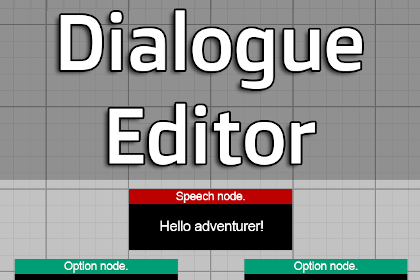
\includegraphics[width=250pt, keepaspectratio]{img/CardImage.png}
\end{figure}

% Links
\section{Links}
\begin{itemize}
\setlength\itemsep{1pt}
	\item \href{https://assetstore.unity.com/packages/tools/utilities/dialogue-editor-168329}{Asset store}
	\item \href{https://www.youtube.com/playlist?list=PLfRF6lnXtGqjrhzyQhidqMD-shMHGReXi}{Video Tutorial Playlist}
\end{itemize}


% Sections
\section{Tutorial}
\begin{itemize}
\setlength\itemsep{1pt}
	\item \hyperlink{_whatis}{What is Dialogue Editor?}
	\item \hyperlink{_editorwindow}{Editor Window}
	\item \hyperlink{_conversationmanager}{Conversation Manager UI Prefab}
	\item \hyperlink{_triggering}{Triggering a conversation}
	\item \hyperlink{_custominput}{Custom Input}
	\item \hyperlink{_callbacks}{Callbacks}
	\item \hyperlink{_datastructure}{Conversation Datastructure}
\end{itemize}


% What is Dialogue Editor
\section{What is Dialogue Editor?}
\hypertarget{_whatis}{}
Dialogue Editor is a Unity tool that allows you to quickly and easily add conversations into your game.
\newline
The tool comes with an editor window that allows you to create and edit conversations.
\newline
This tool also comes with a pre-made, customisable UI prefab so that no UI programming is required. However, if you are comfortable with programming and wish to create your own UI implementation, each conversation can be accessed as a simple data structure.
\newpage


% Editor Window
\section{Editor Window}
\hypertarget{_editorwindow}{}

\subsection{Intro}
Conversations are made up of Speech nodes and Option nodes. Speech nodes represent something a character will say, and Option nodes represent the options available to the player. The connections between these nodes show the flow of the conversation. 

\begin{figure}[ht]
\centering
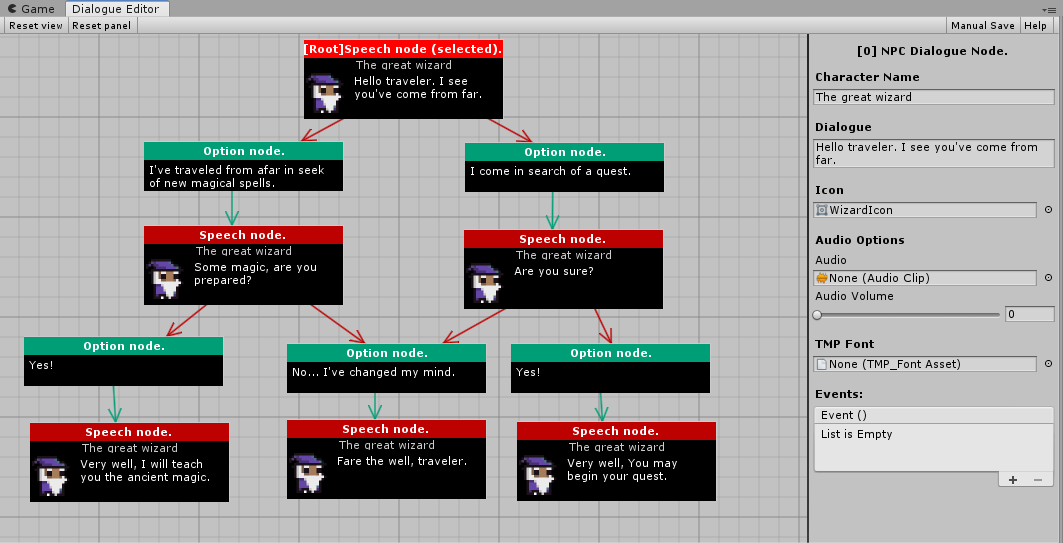
\includegraphics[width=0.8\textwidth, keepaspectratio]{img/EditorWindowFullConversation.png}
\end{figure}


\subsection{Creating a Conversation Object}
In order to create a conversation, create a new GameObject and add the script NPCConversation. 

\begin{figure}[ht]
\centering
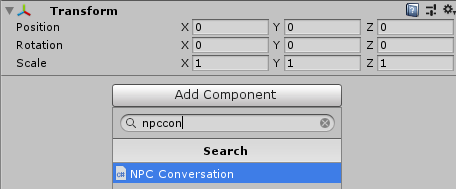
\includegraphics[width=300pt, keepaspectratio]{img/AddNpcConversation.png}
\end{figure}



\subsection{Opening the Editor Window}
In order to open the Editor Window, select Window $\rightarrow$ DialogueEditor. Select a conversation in the hierarchy in order to edit the conversation in the editor window.

\begin{figure}[h]
\centering
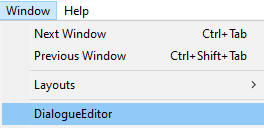
\includegraphics[width=200pt, keepaspectratio]{img/OpenEditorWindow.png}
\end{figure}

\newpage

\subsection{Speech Nodes}
When you create a new conversation, it will contain a single speech node - this is the beginning of the conversation. 
\newline
Click on a speech node to edit it. A speech node has the following variables:
\bigskip

% MINI PAGE - List

\begin{minipage}[c]{0.45\textwidth}
\begin{itemize}
\setlength\itemsep{1pt}
	\item \textbf{Character Name}: This is the name of the character who is speaking.
	\item \textbf{Dialogue}: This is the speech for the node.
	\item \textbf{Automatically Advance}: This option is available if a speech node leads onto another speech node, or nothing. When this option is selected, the dialogue will automatically continue without the user needing to click anything.
	% sub-list
	\begin{itemize}
		\item \textbf{Display Continue Options}: Should the "Continue" / "End" options still display?
		\item \textbf{Dialogue Time}: How long to wait before the dialogue automatically advances.
	\end{itemize}
	\item \textbf{Icon}: This is the icon of the NPC that will appear next to the speech.
	\item \textbf{Audio}: This is an optional variable, you can play audio with this speech.
	\item \textbf{TMPFont}: This is the TextMeshPro font for this speech. You are able to set fonts on a node-by-node basis.
	\item \textbf{Events}: These are Unity Events that will run when this speech node in a conversation is played.
\end{itemize}
\end{minipage}
\hfill
% MINI PAGE - image
\begin{minipage}[c]{0.45\textwidth}
\centering
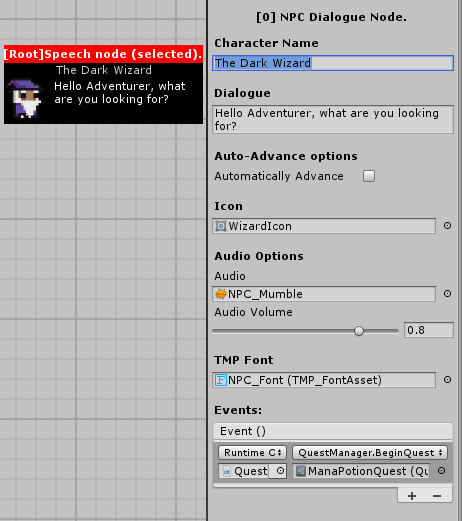
\includegraphics[width=\linewidth]{img/SpeechNode.png}
\end{minipage}




\newpage

\subsection{Option Nodes}
An Option Node represents an option that a user can select.
\newline
Click on an option node to edit it. An option node has the following variables:

\begin{itemize}
\setlength\itemsep{1pt}
	\item \textbf{Option text}: This is the text for the option.
	\item \textbf{TMP Font}: This is the TextMeshPro font that the option text will use.
\end{itemize}

\subsection{Connecting Nodes}
TODO.

\subsection{Deleting Nodes and Connections}
Unwanted connections between nodes can be deleted by right-clicking on the arrow and clicking "Delete this connection"
\newline
Likewise, unwanted nodes can also be deleted by right-clicking on the node and clicking "Delete this node". Deleting a node will also delete any connection to and from this node.
\bigskip 

\begin{minipage}[c]{0.45\textwidth}
\centering
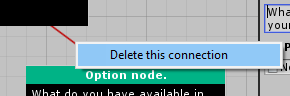
\includegraphics[keepaspectratio]{img/DeleteConnection.png}
\end{minipage}
\hfill
\begin{minipage}[c]{0.45\textwidth}
\centering
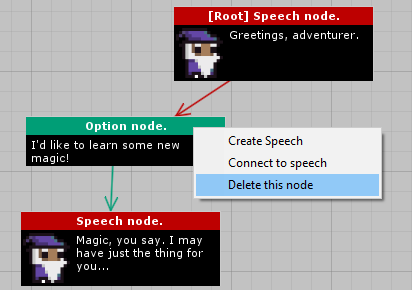
\includegraphics[width=200pt, keepaspectratio]{img/DeleteNode.png}
\end{minipage}




\subsection{Parameters and Conditions}
TODO.

\newpage


% Conversation Manager 
\section{Conversation Manager}
\hypertarget{_conversationmanager}{}
A pre-made, customisable UI prefab is provided. The ConversationManager prefab can be dragged as a child of a Canvas. 
\newline
Recommended settings:
\begin{itemize}
\setlength\itemsep{1pt}
	\item \textbf{Canvas - Render Mode}: Screen Space - Overlay
	\item \textbf{Canvas Scaler - UI Scale Mode}: Scale with Screen Size
\end{itemize}

\begin{figure}[h]
\centering
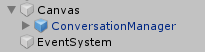
\includegraphics[keepaspectratio]{img/CanvasInHierarchy.png}
\end{figure}

\begin{figure}[h]
\centering
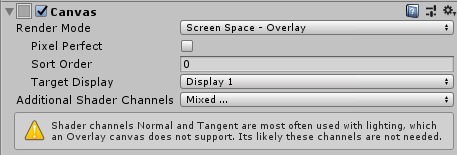
\includegraphics[width=250pt, keepaspectratio]{img/CanvasComponent.png}
\end{figure}


\begin{figure}[h]
\centering
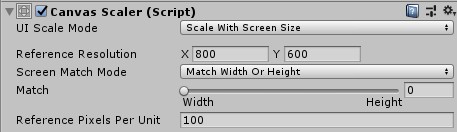
\includegraphics[width=250pt, keepaspectratio]{img/CanvasScalarComponent.png}
\end{figure}

The ConversationManager provides options for the Background image of the Dialogue box and the Options box. These images can be optionally 9-sliced images. A preview render is displayed above the options. You can also select text-scrolling options.

\begin{figure}[h]
\centering
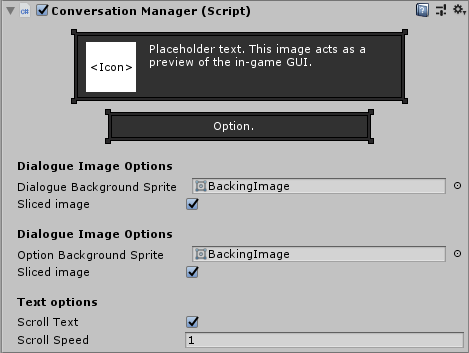
\includegraphics[width=300pt, keepaspectratio]{img/ConversationManager.png}
\end{figure}

\newpage





% Triggering a conversation
\section{Triggering a Conversation}
\hypertarget{_triggering}{}

If you are using the ConversationManager UI Prefab, conversations can be triggered by calling a single function:
\bigskip

\begin{lstlisting}
ConversationManager.Instance.StartConversation();
\end{lstlisting}
\bigskip

Note: You will need to add the "DialogueEditor" namespace to your script. This can be done by adding the following line at the top:
\bigskip

\begin{lstlisting}
using DialogueEditor;
\end{lstlisting}
\bigskip

Here is some example code, which shows a very basic NPC class which begins a conversation when the NPC is clicked on:
\bigskip

\begin{lstlisting}
using UnityEngine;
using DialogueEditor;

public class NPC : MonoBehaviour
{
	public NPCConversation Conversation;

	private void OnMouseOver()
	{
		if (Input.GetMouseButtonDown(0))
		{
			ConversationManager.Instance.StartConversation(Conversation);
		}
	}
}
\end{lstlisting}
\bigskip


There are also a number of additional Properties and Functions available to you:
\bigskip

\begin{lstlisting}
// Is a conversation currently happening?
ConversationManager.Instance.IsConversationActive;

// The current conversation (null if no conversation active).
ConversationManager.Instance.CurrentConversation;

// End a conversation early (e.g. player walks off).
ConversationManager.Instance.EndConversation();
\end{lstlisting}


\newpage











% Custom Input
\section{Custom Input}
\hypertarget{_custominput}{}
Dialogue Editor provides some basic functions which allows you to interact with the Conversation UI. This enables you to support any input method that your game supports, such as Keyboard + Mouse or a Controller
\newline
Three basic functions allow you to cycle to the next or previous option, and to press the currently selected option:
\bigskip

\begin{lstlisting}
// Cycle to the previous option
ConversationManager.Instance.SelectPreviousOption();
// Cycle to the next option
ConversationManager.Instance.SelectNextOption();
// Press the currently selected option
ConversationManager.Instance.PressSelectedOption();
\end{lstlisting}
\bigskip

Here is some example code which shows keyboard support for the Conversation UI:
\bigskip

\begin{lstlisting}
Using UnityEngine;
Using DialogueEditor;

public class ExampleInputManager : MonoBehaviour
{
	private void Update()	
	{
		if (ConversationManager.Instance != null)
		{
			if (ConversationManager.Instance.IsConversationActive)
			{
				if (Input.GetKeyDown(KeyCode.UpArrow))
					ConversationManager.Instance.SelectPreviousOption();
					    
				else if (Input.GetKeyDown(KeyCode.DownArrow))
					ConversationManager.Instance.SelectNextOption();
					
				else if (Input.GetKeyDown(KeyCode.F))
					ConversationManager.Instance.PressSelectedOption();
			}
		}
	}
}
\end{lstlisting}
\bigskip

There is also an option on the Conversation Manager prefab which allows you to choose whether or not mouse interaction should be enabled.

\begin{figure}[ht]
\centering
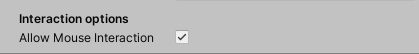
\includegraphics[keepaspectratio]{img/AllowMouseInteraction.png}
\end{figure}

\newpage

% Callbacks
\section{Callback}
\hypertarget{_callbacks}{}

If you are using the ConversationManager UI Prefab, there are two callbacks you can use which are invoked when a conversation starts and ends, respectively.
\bigskip

\begin{lstlisting}
DialogueEditor.ConversationManager.OnConversationStarted
DialogueEditor.ConversationManager.OnConversationEnded
\end{lstlisting}
\bigskip

Note: You will need to add the "DialogueEditor" namespace to your script. This can be done by adding the following line at the top:
\bigskip

\begin{lstlisting}
using DialogueEditor;
\end{lstlisting}
\bigskip

Example use-case:
\bigskip

\begin{lstlisting}
using UnityEngine;
using DialogueEditor;

public class ExampleClass : MonoBehaviour
{
	private void OnEnable()
	{
		ConversationManager.OnConversationStarted += ConversationStart;
		ConversationManager.OnConversationEnded += ConversationEnd;
	}
	
	private void OnDisable()
	{
		ConversationManager.OnConversationStarted -= ConversationStart;
		ConversationManager.OnConversationEnded -= ConversationEnd;
	}
	
	private void ConversationStart()
	{
		Debug.Log("A conversation has began.");
	}
	
	private void ConversationEnd()
	{
		Debug.Log("A conversation has ended.");
	}
}
\end{lstlisting}

\newpage

% Datastructure
\section{Conversation Datastructure}
\hypertarget{_datastructure}{}

If you wish to write your own custom UI, and only use the editor-window for creating the conversation object, the conversation object can be deserialized into a simple and easy-to-use datastructure.

Note: You will need to add the "DialogueEditor" namespace to your script. This can be done by adding the following line at the top:
\bigskip

\begin{lstlisting}
using DialogueEditor;
\end{lstlisting}
\bigskip

In order to deserialize the conversation, NPCConversation contains a function for doing so: this returns an object of type "Conversation":
\bigskip

\begin{lstlisting}
NPCConversation NPCConv;
Conversation conversation = NPCConv.Deserialize();
\end{lstlisting}
\bigskip

A NPCConversation deserializes into a tree-like data structure. A "Conversation" object contains a single member which is the root speech node of the conversation. From here, the nodes are connected in a tree-like pattern. The following classes make up the tree-like structure of a Conversation:
\bigskip

\begin{lstlisting}
public class Conversation
{
	public SpeechNode Root;
}

public abstract class ConversationNode
{
	// The main body text
	public string Text;
	
	public TMPro.TMP_FontAsset TMPFont;
}

public class SpeechNode : ConversationNode
{
	// The name of the speaker
	public string Name;
	
	// Should this dialogue node automatically advance?
	public bool AutomaticallyAdvance; 
	
	// Should the "Continue" / "End" buttons still be visible?
	public bool AutoAdvanceShouldDisplayOption; 
	
	// How long to wait before advancing
	public float TimeUntilAdvance; 
	
	// The Icon of the spaker
	public Sprite Icon;
	
	// Audio to play
	public AudioClip Audio;
	
	// Normalised volume, 0-1, of the audio
	public float Volume;
	
	// The Options available on this Speech node, if any.
	public List<OptionNode> Options;
	
	// The Speech node following this, if any.	
	public SpeechNode Dialogue; 
	
	// The UnityEvent
	public UnityEngine.Events.UnityEvent Event;
}

public class OptionNode : ConversationNode
{
	// The dialogue following this option.
	public SpeechNode Dialogue;
}
\end{lstlisting}


\newpage





\end{document}